% Компіляція: lualatex -shell-escape main.tex
\documentclass[12pt,a4paper]{article}
\usepackage{fontspec,polyglossia}\setdefaultlanguage{ukrainian}\setmainfont{NewComputerModern10}\setmonofont{Noto Sans Mono}[Scale=.82]
\usepackage{amsmath,booktabs,caption,enumitem,float,fvextra,geometry,graphicx,hyperref,microtype,tikz,titlesec}
\usetikzlibrary{arrows.meta,positioning}
\geometry{left=2cm,right=2cm,top=2cm,bottom=2cm}\setlength{\parindent}{1.25cm}\setlength{\parskip}{0pt}\linespread{1.0}\setlength{\emergencystretch}{3em}
\captionsetup{font=small,labelfont=bf,labelsep=endash}
\titleformat{\section}{\normalfont\fontsize{14}{16}\selectfont\bfseries\centering}{\thesection.}{.6em}{}
\titleformat{\subsection}{\normalfont\fontsize{12}{14}\selectfont\bfseries\centering}{\thesubsection.}{.6em}{}
\begin{document}\pagenumbering{gobble}
\begin{titlepage}
\begin{center}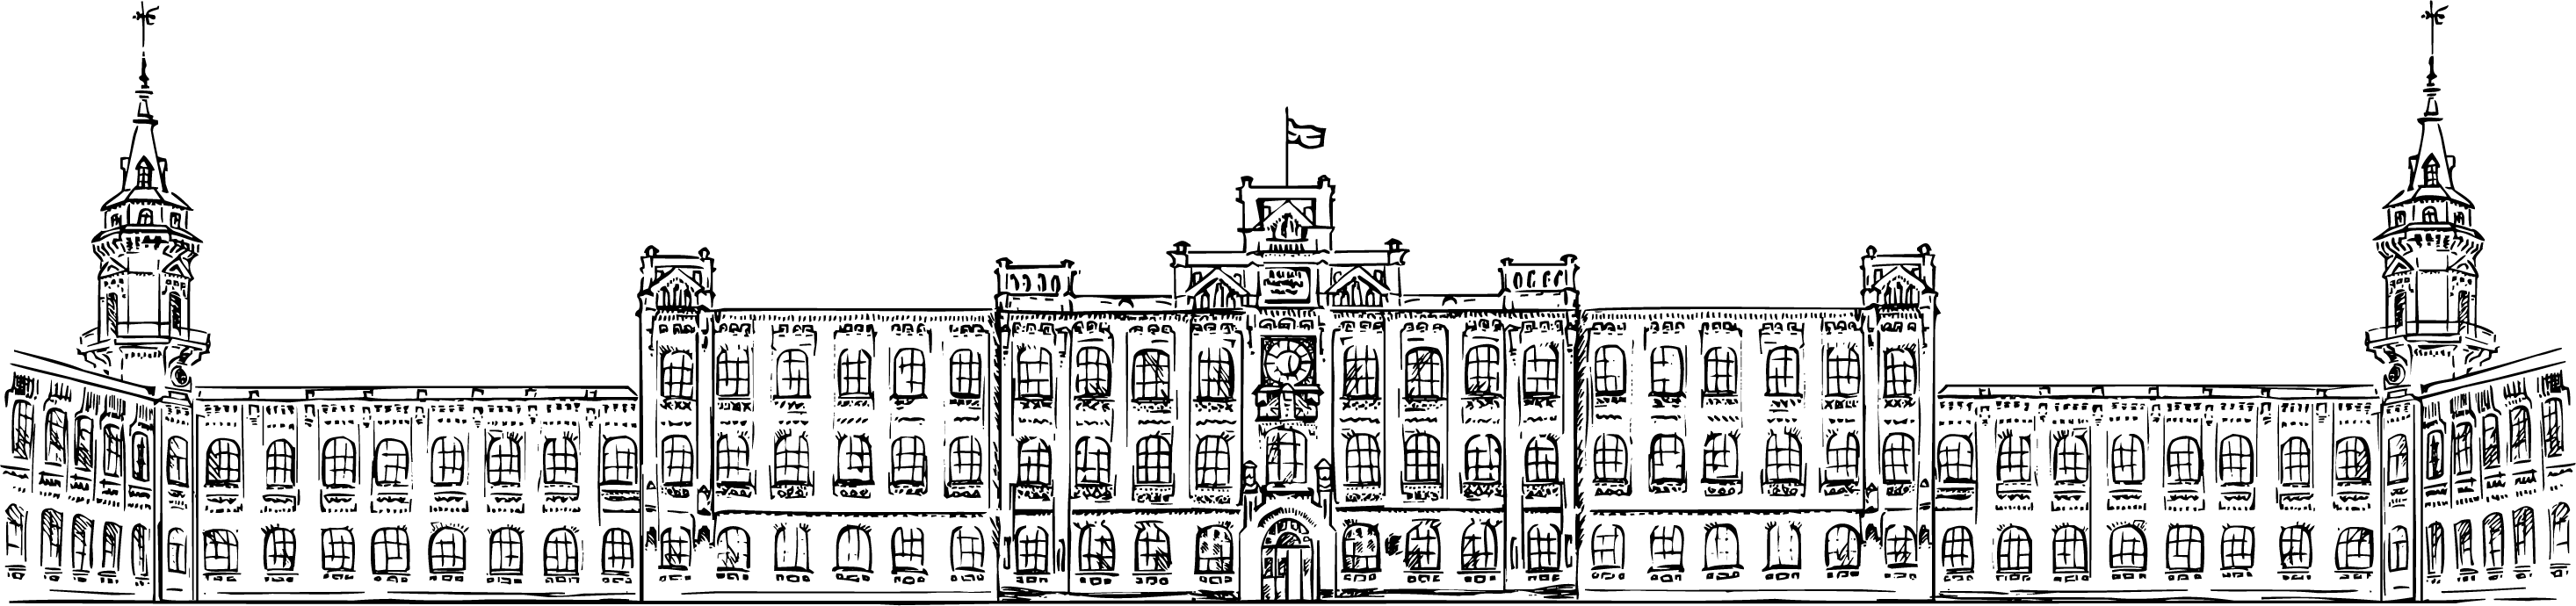
\includegraphics[width=.7\textwidth]{../../../../../../templates/letterhead.png}\end{center}
\begin{center}\large Національний технічний університет України\\«Київський політехнічний інститут імені Ігоря Сікорського»\\[1em]Факультет інформатики та обчислювальної техніки\\Кафедра обчислювальної техніки\end{center}
\vfill\begin{center}\textbf{\LARGE Технології Computer Vision}\\[2em]\textbf{\Large Лабораторна робота №7}\\[.7em]«Реалізація методів глибинного навчання в Computer Vision»\end{center}
\vfill\begin{flushright}\begin{minipage}{.48\textwidth}Виконав: студент 3 курсу ФІОТ,\\групи ІО-41\\\textit{Давидчук А. М.}\\Залікова книжка № 4106\\[1em]Перевірив: \textit{Баран Д. Р.}\end{minipage}\end{flushright}
\vfill\begin{center}Київ --- 2026\end{center}\end{titlepage}
\pagenumbering{arabic}

\section{Тема та мета роботи}
\noindent\textbf{Тема:} штучні нейронні мережі для ідентифікації об'єктів на цифрових зображеннях.

\medskip\noindent\textbf{Мета:} підготувати дані, синтезувати архітектуру, навчити нейромережу та перевірити її застосування у задачі розпізнавання.

\section{Завдання роботи}
Виконується варіант 9: розробити програмний скрипт, що забезпечує ідентифікацію бінарних зображень шести спеціальних знаків, заданих матрицею растра. Нейромережу потрібно синтезувати, навчити й застосувати у ``сирому'' вигляді матричних операцій, обґрунтувати архітектуру й довести працездатність.

Обрані класи: плюс, косий хрест, квадрат, трикутник, коло та стрілка. Розмір растра --- $16\times16$.

\section{Математична модель}
Вхід $x\in[0,1]^{256}$ подається до прихованого шару з 64 нейронами:
\begin{align}
z_1&=xW_1+b_1, & h&=\operatorname{ReLU}(z_1),\\
z_2&=hW_2+b_2, & p_k&=\frac{e^{z_{2k}}}{\sum_j e^{z_{2j}}}.
\end{align}
Функція втрат для мініпакета:
\begin{equation}L=-\frac1N\sum_{i=1}^{N}\log p_{i,y_i}.\end{equation}
Похибки поширюються у зворотному напрямі за правилом ланцюга, після чого ваги оновлюються градієнтним спуском $W\leftarrow W-\eta\nabla_WL$, де $\eta=0{,}12$.

Для кожного класу сформовано 320 прикладів шляхом зсуву еталона до двох пікселів, додавання гаусового шуму та випадкової інверсії 1,5\% пікселів. 80\% даних використано для навчання, 20\% --- для незалежного тесту.

\section{Архітектура рішення}
\begin{figure}[H]\centering
\begin{tikzpicture}[node distance=.65cm,block/.style={draw,rounded corners,align=center,minimum width=2.8cm,minimum height=.8cm,fill=blue!7},arrow/.style={-{Latex},thick}]
\node[block](a){6 еталонів\\$16\times16$};\node[block,right=of a](b){Аугментація\\1920 прикладів};\node[block,right=of b](c){MLP\\256--64--6};
\node[block,below=of c](d){Backpropagation\\180 епох};\node[block,left=of d](e){Тестова вибірка\\384 приклади};\node[block,left=of e](f){Accuracy і\\матриця помилок};
\draw[arrow](a)--(b)--(c)--(d)--(e)--(f);
\end{tikzpicture}\caption{Блок-схема навчання та перевірки}
\end{figure}

\section{Результати}
\begin{figure}[H]\centering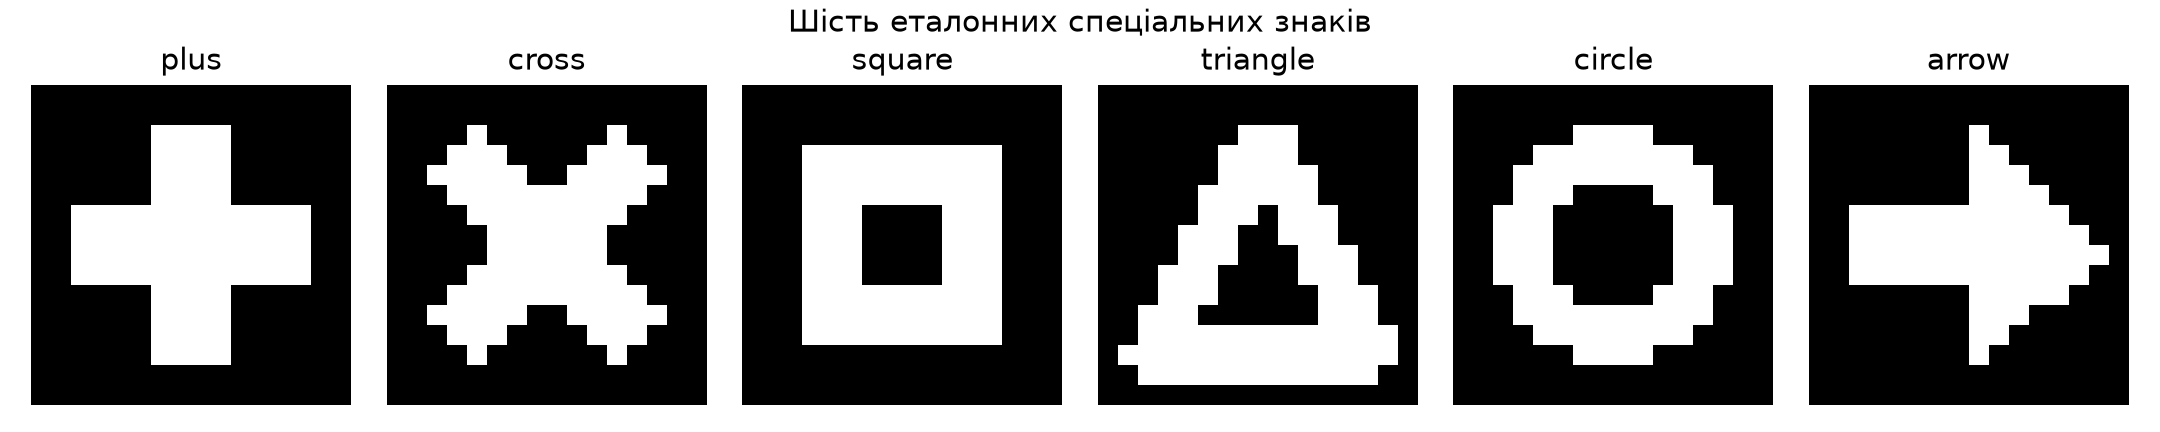
\includegraphics[width=.95\textwidth]{../results/templates.png}\caption{Еталонні бінарні знаки}\end{figure}
\begin{figure}[H]\centering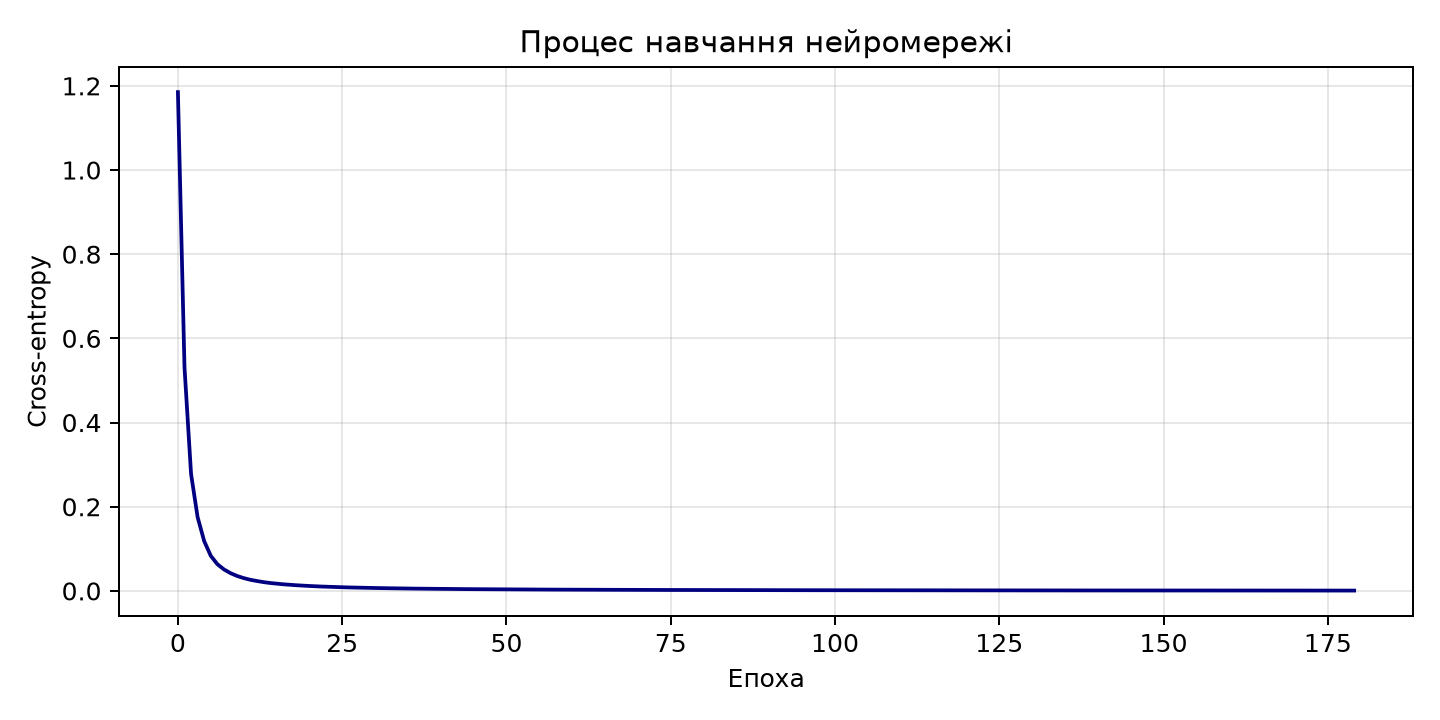
\includegraphics[width=.82\textwidth]{../results/training_curve.png}\caption{Зменшення функції втрат}\end{figure}
\begin{table}[H]\centering\caption{Параметри та результати експерименту}
\begin{tabular}{lr}\toprule Показник&Значення\\\midrule Навчальних прикладів&1536\\Тестових прикладів&384\\Епох&180\\Фінальна cross-entropy&0,000789\\Точність&1,000000\\\bottomrule\end{tabular}
\end{table}
\begin{figure}[H]\centering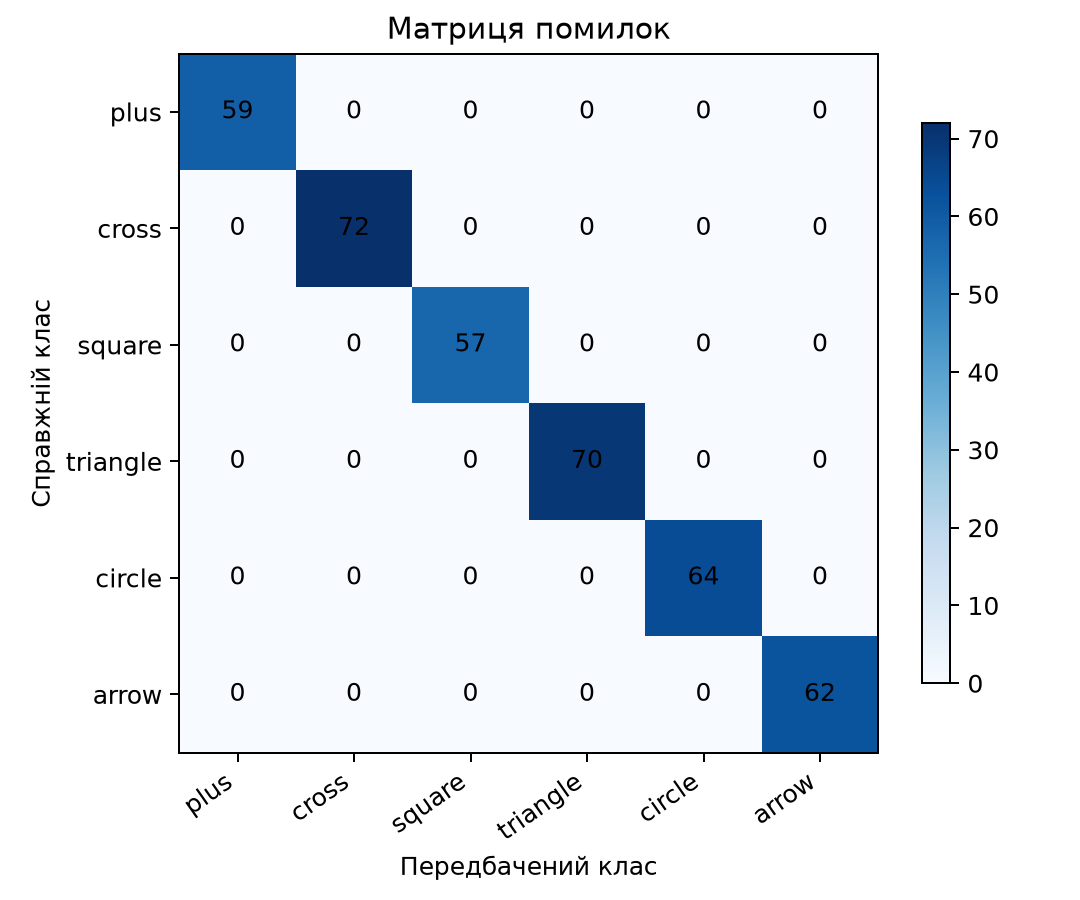
\includegraphics[width=.75\textwidth]{../results/confusion_matrix.png}\caption{Матриця помилок на тестовій вибірці}\end{figure}
\begin{figure}[H]\centering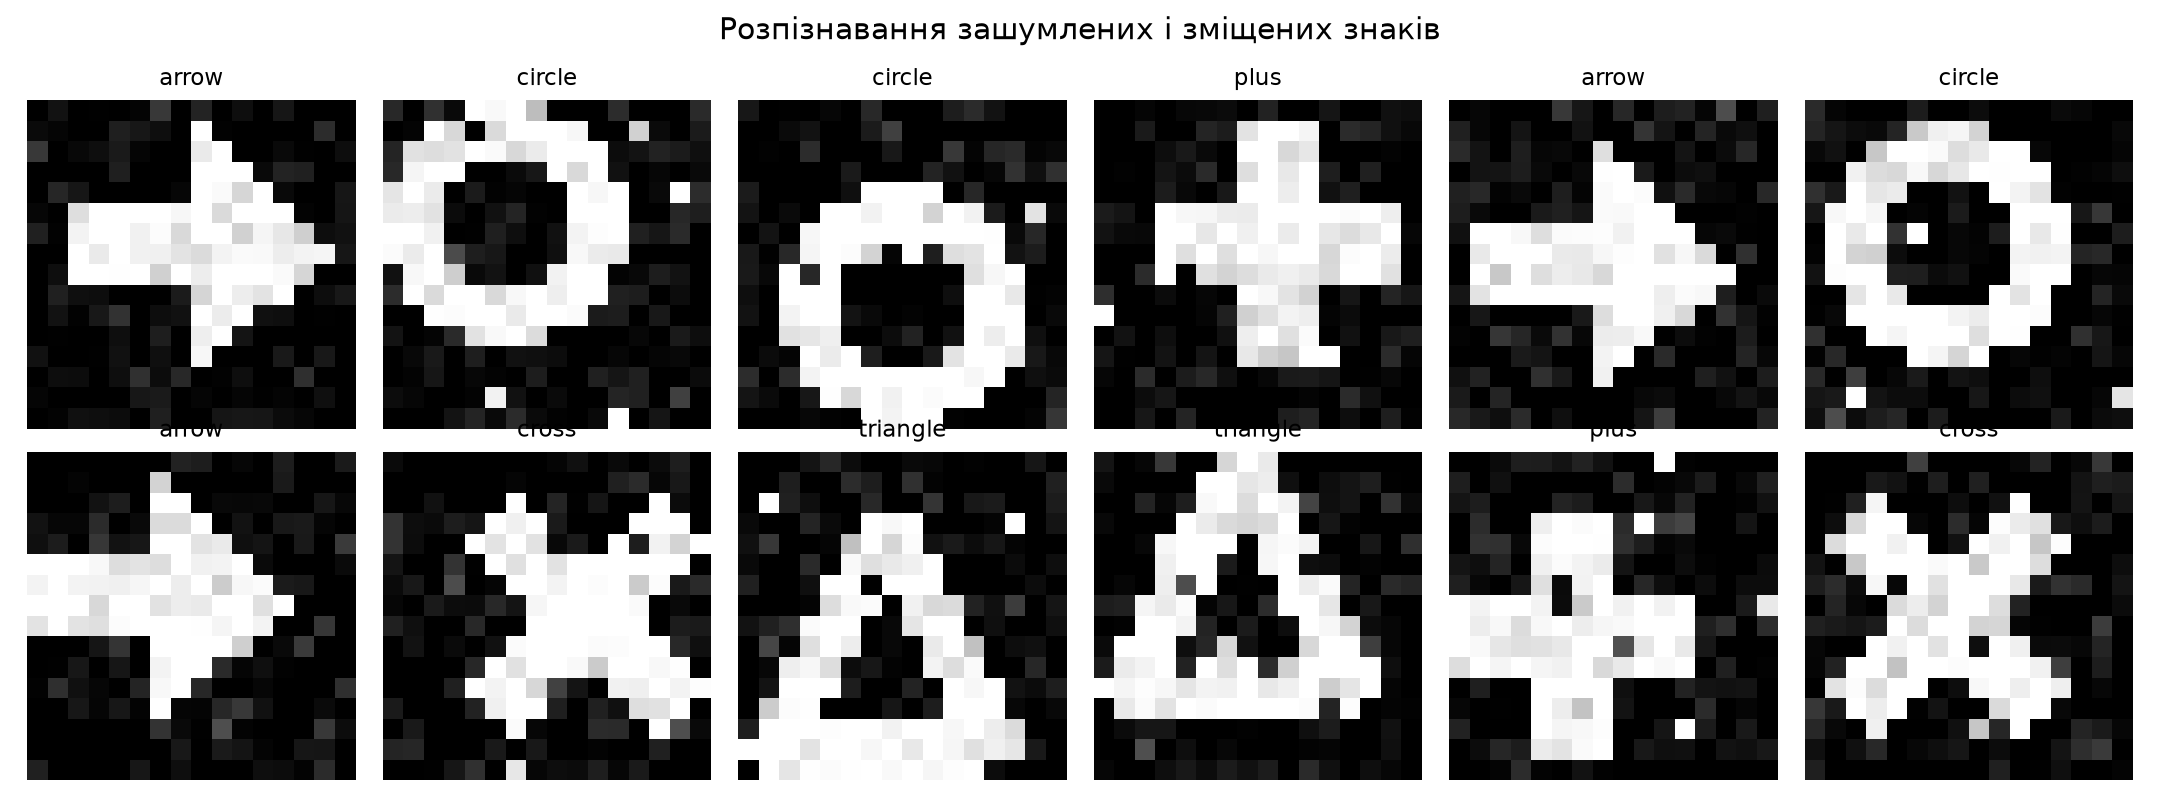
\includegraphics[width=.98\textwidth]{../results/predictions.png}\caption{Приклади розпізнавання зашумлених знаків}\end{figure}
Нульові позадіагональні елементи матриці помилок означають, що всі 384 тестові приклади розпізнані правильно. Модель та назви класів збережено у \texttt{model.npz}.

\section{Структура проєкту}
\begin{verbatim}
lab7/
|-- src/main.py
|-- results/model.npz, metrics.csv, *.png
|-- requirements.txt
`-- docs/main.tex, main.pdf
\end{verbatim}

\section{Висновки}
Варіант 9 виконано без високорівневих ML-фреймворків: прямий і зворотний проходи реалізовано матричними операціями NumPy. Архітектура 256--64--6 має достатню місткість для шести геометрично різних класів і досягла 100\% точності на відкладеній вибірці. Висока точність стосується синтетичного розподілу зсувів і шумів; для реальних знаків потрібні різноманітніші дані.

\section{Лістинг програми}
\VerbatimInput[fontsize=\small,numbers=left,breaklines=true,frame=single]{../src/main.py}
\end{document}
